\chapter{Fundamentals of probability and statistics}
\section*{Probability}
	Considering an experiment with random outcomes, a \textbf{event} is defined \textit{as a set of the outcomes of the experiment}, so an event occurs if the outcome of the experiment in one of the element of the set itself. By this concept we can define the \textbf{probability} $\prob{A}$ of the event $A$ as a measure that always satisfies the \textbf{three axioms of probability}:
	\begin{enumerate}
		\item $\prob{A} \geq 0$;
		\item $\prob S = 1$  if $S$ is the sure event;
		\item if two events $A,B$ such that $A \cap B = \emptyset$, or in other word they are \textit{mutually exclusive}, than $\prob{A \cup B} = \prob{A+B} = \prob A + \prob B$.
	\end{enumerate} 

	As a consequence of the last axiom, by defining $\overline A$ the \textbf{complementary event} of $A$, the respective probability is defined as $\prob{\overline A} = 1 - \prob A \leq 1$. In particular the probability of the impossible event (so $\overline S$), expressed by the empty set $\emptyset$, is evaluated as $\prob\emptyset = 0$. Any possible event is a subset of the sure event.
	
	There are usually two different views of probability:
	\begin{itemize}
		\item the \textbf{frequentist} interpretation for which the probability of something corresponds to what fraction of the time it happens \textit{"in the long run"};
		\item the \textbf{Bayesian} interpretation instead considers the probability of something corresponds to how likely we \textit{"think"} it is to happen.
	\end{itemize}
	The \textbf{relative frequency} is a non-rigorous way to introduce the concept of probability with is widely used in engineering system. Considering for example the experiment of tossing a coin (which the associated event are a head $C$ o a tail $\overline C$) and extracting a red/black card from a card deck (so the events are $R$ for the red card and $\overline R$ for the black one). At this point we can describe the sure event as the sum of all the possible outcomes of these experiment, so
	\[ S = \big\{ CR, C\overline R, \overline C R, \overline C \overline R \big\}\]
	After $n$ experiments it is possible to calculate the relative frequency $f(\cdot)$ of a event simply by dividing the number of outcomes $n_i$ in that specific set respect to $n$ itself:
	\[ f\big( CR \big) = \frac{n_1}{n} \qquad f\big( C \overline R \big) = \frac{n_2}{n} \qquad f\big( \overline CR \big) = \frac{n_3}{n} \qquad f\big( \overline C \overline R \big) = \frac{n_4}{n} \qquad  \] 
	
	From an empirical definition we can calculate the probability of tossing a head \textbf{or} extracting a red card by summing the probabilities of the mutually exclusive events that satisfies at least one of the mentioned requisites, so
	\[ f\big(C+R\big) = F \big( CR\big) + f\big(C \overline R\big) + f\big(\overline C R\big) = \frac{n_1 + n_2 + n_3}{n}\]
	Considering that the probability of tossing a head and the probability of extracting a red card are described by the equations
	\[ f\big(C\big) = f\big(CR\big) + f\big(C\overline R\big) = \frac{n_1+n_2}{n} \qquad f\big(R\big) = f\big(CR\big) + f\big(\overline C R\big) = \frac{n_1+n_3}{n} \]
	it's also possible to notice that
	\[ f\big(C+R\big) = \frac{n_1+n_2+n_3 + n_1 - n_1}{n} = f\big(C\big) + f\big(R\big) - f\big(CR\big)\]
	This relation can also be expressed only using the third axiom of probability and so $\prob{C\cup R} = \prob C + \prob R - \prob{C\cap R}$.
	\vspace{3mm}
	
	In general the probability of an event can be effected by an \textit{a-priori} knowledge of some result of the experiment; using the same example as before we can evaluate the probability $f\big(C|R\big)$ of tossing a head knowing that the event $R$ (red card extracted) has been already verified by using the following rule:
	\[ f\big(C|R\big) = \frac{n_1}{n_1+n_3} = \frac{n_1}{n} \frac{n}{n_1+n_3} = \frac{f(CR)}{f(R)} \]
	Similarly we can define the relative frequency $f\big(R|C\big)$ of $R$ knowing $C$ as $f\big(CR\big)/f\big(C\big)$; using the axiom of probability we can define the \textbf{conditional probability} as
	\[ \prob{C|R} = \frac{\prob{C\cap R}}{\prob R}\]
	By inverting this relation it's possible to write the probability of a red card and a head toss, and so
	\[ \prob{C \cap R} = \prob{C|R} \prob{R} = \prob{R|C} \prob C\]
	As consequence if $C$ and $R$ are two statistically independent events, the conditional probability $\prob{C|R}$ corresponds only to the events associated to a head coin toss, and so
	\[ \prob{C\cap R} = \prob C \prob R \]
	
	In general given two events $A,B$, as expressed before their conditional probability is described by the equation $\prob{A \cup B} = \prob{A|B} \prob B = \prob{B|A} \prob A$. By manipulating this relation it's possible to describe the conditional probability $A|B$ in relation to the other conditional probability $B|A$ by simply doing
	\[\prob{A|B} = \prob{B|A} \frac{\prob A}{\prob B} \]
	So given $n$ disjoint events $A_i$ (with $i$ that goes from 1 to $n$) it's possible to express the conditional probability $A_i|B$ of one event in respect to $B$ by using the \textbf{Bayes theorem} which states that
	\[ \prob{A_i|B}  = \prob{B|A_i} \frac{\prob{A_i}}{\prob B} =  \frac{\prob{B|A_i} \prob{A_i}}{\sum_{j=1}^n \prob{B|A_j}\prob{A_j}} \]
	In respect to this theorem we can see three main component:
	\begin{itemize}
		\item $\prob {A_i}$ is the \textit{prior probability} of the event $A_i$;
		\item $\prob{B|A_i}$ is the \textit{likelihood} of $B$ given $A_i$, so it's a measure of how likely $B$ happens when $A_i$ also happens;
		\item $\prob{A_i|B}$ is the \textit{posterior probability} of $A_i$ given $B$ (the probability of $A_i$ knowing that $B$ has actually happened).
	\end{itemize}

\section*{Random variables}
	In the majority of the engineering cases the variables are not described by set of events but with numbers. In general a \textbf{random variable} is a real-valued function that assumes a certain value according to the outcome of a certain random experiment.
	
	To a formal level the random variables maps the set containing all the possible outcomes of a certain experiments, the so called \textit{event/sample space} $\Omega$ (that can be continuous, like $\mathds R$, or discrete, like $\mathds Z$) to the space of numbers. In practise $\forall \omega \in \Omega$ we get that the mapped value $x(\omega)$ is an element of the the arriving set (like a number).	
	\begin{SCfigure}[1.5][bht]
		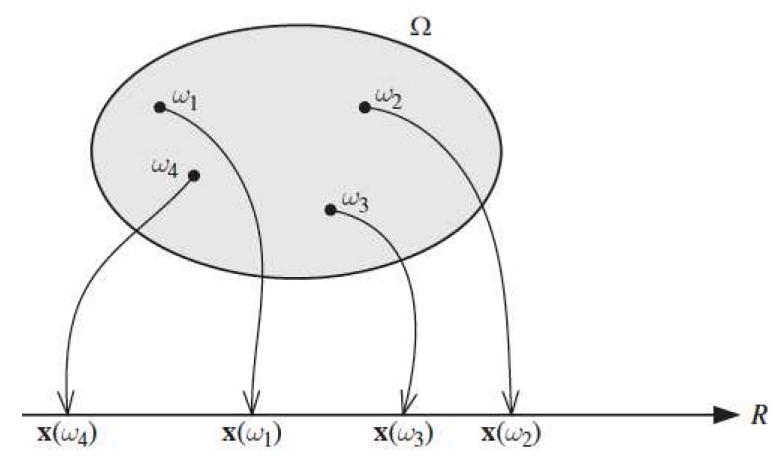
\includegraphics[width=5cm]{randomvariables}
		\caption{example of a random variable being mapped from a sample space $\Omega$ to a continuous set of the real number.}
	\end{SCfigure}
	
	To completely describe a random variable it's necessary to use a probabilistic description, in particular by using the so called \textbf{probability density function} (pdf) that can calculate the probability of a random variable $x$ at a certain value $x=a$ by the formula
	\[ p(a) = \lim_{\delta_a \rightarrow 0} \frac{\prob{a-\delta_a < x \leq a}}{\delta_a} \geq 0 \]
	This expression resembles a derivative: this function can in fact be integrated between two points in order to get the probability of having a random variables inside that range
	\[ \prob{a< x \leq b} = \int_a ^b p(x)\, dx \]
	From the probability density function it can be derived the \textbf{cumulative distribution function} (cdf) that describes the probability of having a random variable $x$ with value less or ugual to $b$:
	\[ P(b) = \prob{x\leq b} = \int_{-\infty}^b p(x)\, dx\]
	
	The pdf associated to a random variable, in order to satisfy the second axiom of probability, must require that
	\[ \prob{x\leq \infty} = \int_{-\infty}^\infty p(x)\, dx = P(\infty) = 1\] 
	\vspace{3mm}
	
	Usually all the probability density functions for continuous random variables can be expressed as a \textit{known distribution} by re-shaping the pdf as
	\[ p(x) = \frac{1}{c\, N(s)} p\left(\frac{x-l}{c}\right)\]
	where $l$ is the \textit{location parameter} (that has the role to translate the pdf), $c$ is the \textit{scale parameter} (associated to a expansion/contraction) and $s$ is a \textit{shape parameter} that governs the shape of the pdf and that define the normalising function $N(s)$.\\
	Examples of known probability density functions is the \textbf{uniform} one; in this case the random variable $x$ comparable to this distribution in the range $[a,b]$ is written as $x\backsim \mathcal U(a,b)$ and in particular
	\[ p(x) = \mathcal U(x; a,b) := \begin{cases}
		\frac 1{b-a} \qquad & \textrm{if } x\in [a,b] \\ 0 & \textrm{otherwise}
	\end{cases} \]
	Another important distribution is the \textbf{normal} $\mathcal N$ (or \textbf{gaussian}) one that requires the definition of all the 3 parameters defined above ($l, c,N(s)$) and the pdf associated is described as
	\[ p(x) = \mathcal N\big(x; l, c, N(s)\big) := \frac{1}{\sqrt{2\pi} c} e^{-\dfrac{(x-l)^2}{2c^2}} \]
	where $N(s)$= $\sqrt{2\pi}$ comes from the normalization of the pdf.
	\vspace{3mm}
	
	The analogous of the pdf for discrete valued variable $a$ is called \textbf{probability mass function} usually described as $\pi(a_i) = \prob{x=a_i} = \pi_i$. Knowing that the random variable has $n$ discrete steps, the following rule must be respected
	\[\sum_{i=1}^n \pi_i = 1\]
	An example of a probability mass function is the \textbf{Poisson} distribution with rate $\lambda$ that's used to calculate the probability of a certain number of random points in an interval $T$:
	\[ \pi(a) = \prob{x=a} = e^{-\lambda t} \frac{\big(\lambda T\big)^a}{a!} \qquad a \in \mathds N_0 \]
	\vspace{3mm}
	
	It is sometimes needed to characterise a random variable with certain attributes like the typical value, the spread or variability od the variable, and so on: this properties are computed on the probability density function of the variable, not non the raw collected data.\\
	In general we might be interested to calculate the \textbf{central value} of a random variable, but this value is'n unique and it depends on the definition adopted
	\begin{itemize}
		\item the \textbf{mode} corresponds to the value associated at the maximum of the pdf, so the most recurring value in the random variable domain; this central value definition isn't the best because in some cases it's possible to have multiple peaks;
		
		\item another way to determine the central value is by using the \textbf{moments} (concept derived by the mechanical world) calculating the $r-th$ moment with respect to the origin $\mu_r'$ or in respect to the mean $c_r'$ (in this case $\mu_1'$ is the mean value of the distribution):
		\[ \mu_r' = \int_{-\infty}^\infty x^r\, p(x)\, dx \qquad c_r' = \int_{-\infty}^\infty \big(x-\mu_1'\big)^r p(x)\, dx \]
		More precisely the moments are defined using the \textbf{expected value} operator $E(x)$ that's defined as
		\[ E(x) := \int_{-\infty}^\infty x p(x)\, dx\]
		By this new definition the $r-th$ moments of the random variables can be expressed as $\mu_r' = E\{x^r\}$ and $c_r' = E \big\{ (x-\mu_1')^r \big\}$. In particular for $r = 0$ no information are retrieved because for each random variable $x$ it happens that $\mu_0' = c_0' = 0$. By choosing $r = $, the value $\mu_1' := \mu$ represent the \textbf{mean} of the random variable, so \textit{the long run average}; calculating the value $c_1'$ gives no additional information ($c_1' = 0 \forall x$). By computing the $2-th$ moment it's possible to define the \textbf{variance} as $\sigma^2 := c_2'$.
	\end{itemize}

	So in general given a random variable $x$ it's possible to compute the mean $\mu$ and the variance $\sigma^2$ by using the following rules:
	\[ \mu = \int_{-\infty}^\infty x p(x)\, dx \qquad \sigma^2 = \int_{-\infty}^\infty \big(x-\mu \big)^2 p(x)\, dx  \]
	Applying this rule to the distributions mentioned before we can calculate the mean and the variance of a uniform distribution $\mathcal U (a,b)$ as $\mu = \frac{b+a}{2}$ and $\sigma^2 = \frac 1 {12} (b-a)^2$. Considering instead the gaussian distribution, the expected value is more complex to calculate, but some step of the demonstration are here described as well as the solution
	\begin{align*}
		E\{x\} = \mu & = \int_{-\infty}^\infty x \frac 1 {\sqrt{2\pi} c} e^{-\frac{(x-l)^2}{2c^2}} \, dx \\ & = \int_{-\infty}^\infty \big(x-l\big) \frac 1 {\sqrt{2\pi} c} e^{-\frac{(x-l)^2}{2c^2}} \, dx + l \int_{-\infty}^\infty x \frac 1 {\sqrt{2\pi} c} e^{-\frac{(x-l)^2}{2c^2}} \, dx \\
		& = \int_{-\infty}^\infty y \frac 1 {\sqrt{2\pi} c} e^{-\frac{y^2}{2c^2}} \, dy + l\\
		& = \int_{-\infty}^0 y \frac 1 {\sqrt{2\pi} c} e^{-\frac{y^2}{2c^2}} \, dy + \int_0^\infty y \frac 1 {\sqrt{2\pi} c} e^{-\frac{y^2}{2c^2}} \, dy + l \\
		& = l
	\end{align*}
	So in this case it's possible to see that the mean of a normal distribution is equal to the location parameter $l$ described by the function, and (as it's going to be demonstrated) the variance is equal to the scale parameter $\sigma^2 = c^2$:
	\begin{align*}
		V\{x\} = \sigma^2 & = E\big\{(x-\mu)^2\big\} = \int_{-\infty}^\infty \big(x-\mu\big)^2 \frac 1 {\sqrt{2\pi} c} e^{-\frac{(x-\mu)^2}{2c^2}} \, dx \\
		& = \int_{-\infty}^\infty y^2 \frac 1 {\sqrt{2\pi} c} e^{-\frac{y^2}{2c^2}} \, dx = c^2
	\end{align*}
	In general the value $\sigma= \sqrt{\sigma^2}$ is defined as \textbf{standard deviation}. In a practical way the mean value gives an idea of the central value of the random variable while the variance represent how much this variable is spread.
	
	Another important way to determine the central value is by computing the \textbf{median} $\tilde \mu$ of a random variable, so by determining the values that satisfies the following equation:
	\[ \int_{-\infty} ^{\tilde \mu} p(x)\, dx = \int_{\tilde \mu}^\infty p(x) \, dx \]
	In general the median is a more robust way to estimate the central value of a random variable and so it's often more used; direct consequence of the median is the \textbf{mean deviation} (concept that replaces the variance) defined as
	\[ \overline \mu = \int_{-\infty}^\infty |x-\mu| p(x)\, dx \]
	
	
	
	
	
	
	
	
	
	
	
	
	
	
	
	
	
	
	
	